\subsection*{Формы воды в почве и их доступность для растений}

\paragraph{}Собственно весь водный обмен в растении состоит из трех основных этапов:

\begin{enumerate}

	\item Поглощения воды из почвы;
	\item Передачи воды из корня ко всем органам растения; 
	\item Испарение воды из листьев;

\end{enumerate}
 
\note{В почве имеются водоудерживающие силы, которые определяют притяжение воды к почвенным частицам, поэтому далеко не вся вода, находящаяся в почве доступна растениям.}


\remember{Почвенный раствор обладает собственной сосущей силой, поэтому механизм поступления воды в растение прежде всего обуславливается разницей между \hyperlink{osmosis}{осмотическим давлением} корневого волоска и почвенного раствора}
	
\paragraph{}Концентрация почвенного раствора зависит от количества солей в почве, механического состава почвы, соотношения минеральных и коллоидных частиц в почве. 

\paragraph{}Вода, находящаяся в почве, в зависимости от своего состояния может находиться в одной из следующих форм:

\begin{enumerate}

	\item \termin{Гравитационная} -- вода, заполняющая большие почвенные капилляры, попадающая в почву при дожде или поливе, быстро двигающаяся вниз в глубокие слои почвы под действием силы тяжести собственного веса. Для растений существенного значения не имеет.

	\item \termin{Капиллярная} -- заполняющая узкие капилляры и удерживающаяся силами поверхностного натяжения менисков. Она находится в почве длительное время, незначительно притягивается к почвенным частицам, является наиболее доступной для растений формой.

	\item \termin{Пленочная} -- покрывающая непосредственно почвенные частицы, удерживающаяся на их поверхности силами молекулярного притяжения или адсорбционными силами почвенных частиц. Эта вода труднодоступна для растений.

	\item \termin{Гигроскопическая} --  находящаяся в воздушно-сухой почве, удерживаемая внутри почвенных частиц силой свыше 100000 кПа. Ее количество колеблется от 5\% в песчаной почве до 14\% в глинистой почве. Для растений эта вода недоступна.

	\item \termin{Имбибиционная} -- это вода, находящаяся внутри коллоидных частиц почвы, вызывающая их набухание, при этом в набухшей коллоидной частице создаются значительные водоудерживающие силы. Эта форма воды характерна для торфяников. Для растений она также практически недоступна.

\end{enumerate}

\paragraph*{}\note{Для различных видов растений (засухоустойчивых или влаголюбивых) оптимальное значение влажности почвы может варьировать в достаточно широких пределах. Семена растений обладают настолько большой сосущей силой, что способны при прорастании даже использовать недоступную гигроскопическую форму воды}

\paragraph*{}\gls{SoilQquantOfWater} -- это величина, количественно характеризующая водоудерживающую способность почвы (это свойство почвы удерживать в себе то или иное количество влаги от стекания действием капиллярных и сорбционных сил).

\paragraph*{}Различают следующие разновидности влагоемкости:

\begin{enumerate}

\item общую, 
\item полную, 
\item капиллярную или относительную, 
\item полевую или предельную или наименьшую, 
\item максимальную молекулярную.

\end{enumerate}

\paragraph*{}Для определения необходимости полива чаще всего используют понятие предельной полевой влагоемкости (ППВ). 

\note{Поливы назначают при показателе влажности почвы равном 70-75\% от предельной полевой влагоемкости}

\paragraph*{}\termin{Полевая или наименьшая} или предельная влагоемкость -- это наибольшее возможное содержание подвешенной влаги в данном слое почвы в ее естественном сложении при отсутствии слоистости и подпирающего действия грунтовых вод, после стекания всей гравитационной влаги.

\paragraph*{}\termin{Коэффициент} завядания для данной почвы -- это такая величина влажности почвы при которой в специально поставленных опытах наступает длительное завядание растения. Этот показатель зависит только от типа почвы. 

\paragraph*{}\note{Чем легче почва (Например, песчаные, супесчаные), тем полнее используется растениями имеющаяся в ней вода, собственная влагоемкость почвы при этом меньше, т.е. меньше воды находится в виде мертвого запаса, недоступного растениям. Наоборот, влагоемкость тяжелых глинистых почв выше, значит и мертвый запас воды в ней больше.}

\subsection*{Поступление воды в растение}

\paragraph*{}Практически вся вода поступает в растение через корневую систему. Корневая система распространяется в почве в вертикальном и горизонтальном направлениях.

\paragraph*{}Так как вы уже должны знать анатомическое строение растения из курса <<Ботаника>>, здесь приводится лишь рисунок анатомического строения корня \ris \ref{root_shema}.

%%%%%%%%%%%%%%%%%%%%%%%%%%%%%%%%%%%%%%%%%%%%%%%%%%%%%%%%%%%%%%%%%%%%%%%%%%%%%%%%%%%%%%%%%%%%%%%%%%%%%%%

\begin{figure}[h]
\begin{minipage}[h]{0.49\linewidth}
\center{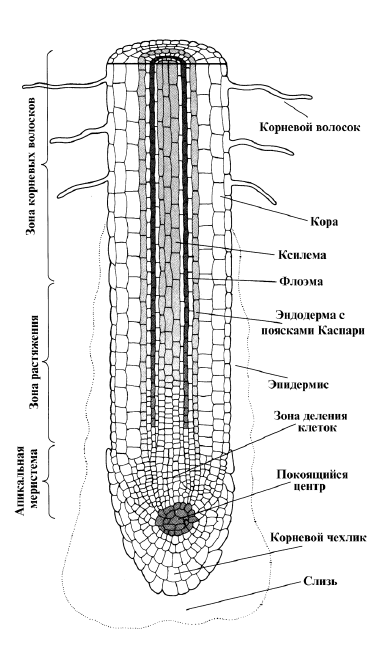
\includegraphics[width=0.8\linewidth]{pictures/root} \\ а) Продольный разрез}
\end{minipage}
\hfill
\begin{minipage}[h]{0.49\linewidth}
\center{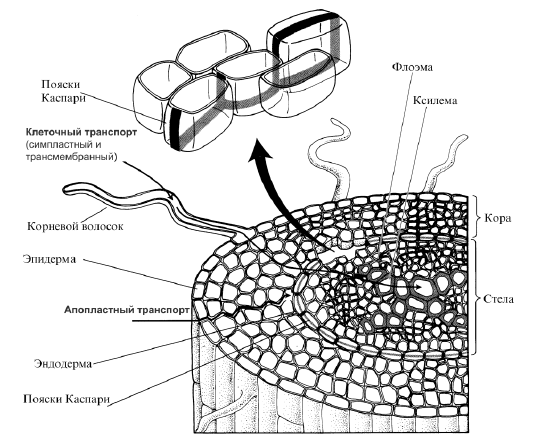
\includegraphics[width=1.2\linewidth]{pictures/root_cross} \\ б) Поперечный разрез}
\end{minipage}
\caption{Схема строения корня}
\paragraph*{}Согласно С.С. Медведева \cite{medvedev_2012}
\label{root_shema}
\end{figure}

%%%%%%%%%%%%%%%%%%%%%%%%%%%%%%%%%%%%%%%%%%%%%%%%%%%%%%%%%%%%%%%%%%%%%%%%%%%%%%

\paragraph*{}Корневая система поглощает воду через корневые волоски, находящиеся в \termin{зоне всасывания}.

\note{Попав в клетку корневого волоска вода становится частью живой системы - клетки растения -- и подчиняется закономерностям, действующим в живой клетке.}

\paragraph*{}Поступление воды в корневую систему растения и перемещение ее по тканям корня осуществляется путем \hyperlink{diffusion}{диффузии}. При этом перемещение воды идет по градиенту ее концентрации.

\paragraph*{}Передвижение по растению определяется двумя основными \termin{двигателями водного потока} в растении:

\begin{enumerate}

\item нижним двигателем водного потока или корневым давлением
\item верхним двигателем водного потока или присасывающим действием атмосферы

\end{enumerate}

\paragraph*{}Действие присасывающей силы корня является причиной таких явлений, как:

\begin{enumerate}

	\item \termin{Гуттация} -- это выделение капельно-жидкой влаги листьями через \termin{гидатоды} в условиях затрудненного испарения (\ris \ref{cry_gutattion} б)
	\item \termin{Плач растения} -- это вытекание \termin{пасоки} (воды с растворенными в ней минеральными веществами, находящейся в ксилеме) из стеблей растений со срезанными побегами (\ris \ref{cry_gutattion} а)

\end{enumerate}

%%%%%%%%%%%%%%%%%%%%%%%%%%%%%%%%%%%%%%%%%%%%%%%%%%%%%%%%%%%%%%%%%%%%%%%%%%%%%%%%%%%%%%%%%%%%%%%%%%%%%%%

\begin{figure}[h]
\begin{minipage}[h]{0.49\linewidth}
\center{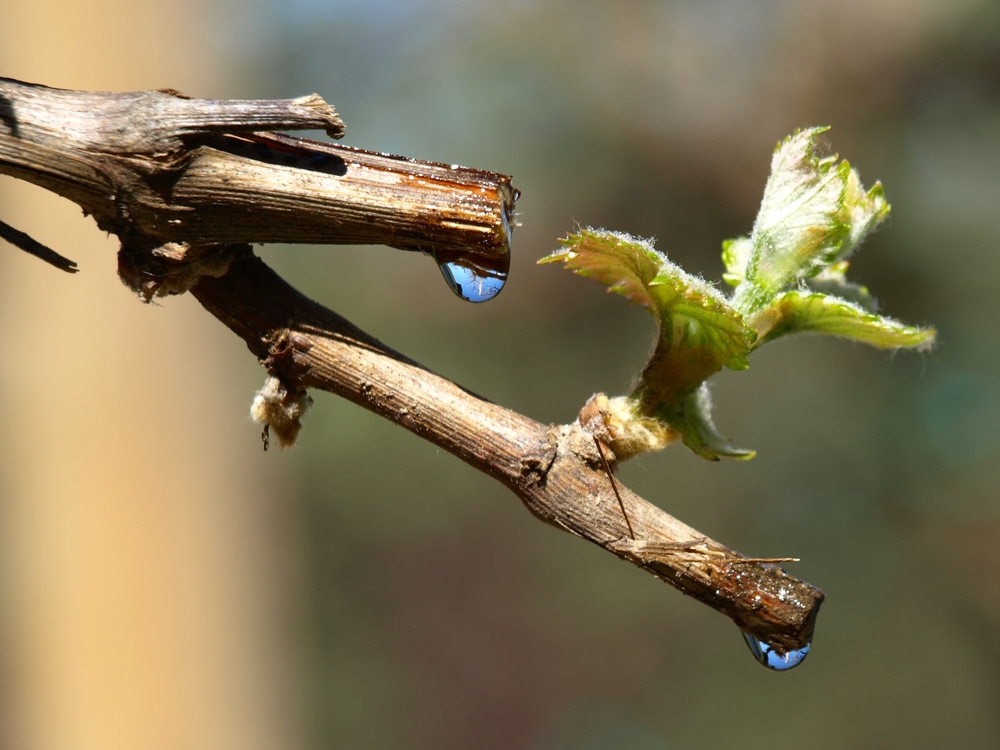
\includegraphics[width=1.1\linewidth]{pictures/cry} \\ а) Плач}
\end{minipage}
\hfill
\begin{minipage}[h]{0.49\linewidth}
\center{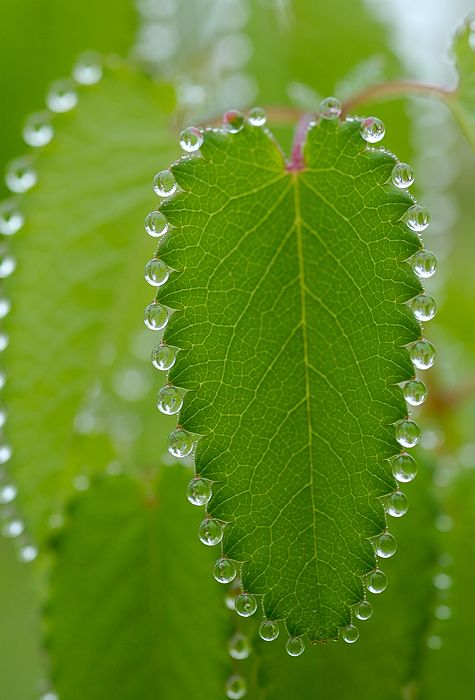
\includegraphics[width=0.55\linewidth]{pictures/guttation} \\ б) Гуттация}
\end{minipage}
\caption{Схема строения корня}

\label{cry_gutattion}
\end{figure}

%%%%%%%%%%%%%%%%%%%%%%%%%%%%%%%%%%%%%%%%%%%%%%%%%%%%%%%%%%%%%%%%%%%%%%%%%%%%%%

\note{Явление гуттации особенно широко распространено в \hyperlink{question_guttation_tropics}{тропиках}, где иногда даже можно попасть под дождь, вызванный гуттирующими растениями \cite{medvedev_2012}}

\note{Состав пасоки сильно варьирует в зависимости от вида растения и фазы его вегетации и фазы органогенеза. Пасока однолетнего травянистого растения и многолетнего древесного растения сильно отличаются друг от друга, так же как и пасока у одного и того же растения весной, летом и осенью. Пасокой являляется березовый сок и кленовый сок. Пасока, выделяющаяся при гуттации, имеет в своем составе очень мало минеральных веществ и сахаров, поскольку происходит их естественная фильтрация при прохождении пасоки через эпитему (ткань, выстилающую воздушную полость гидатоды)}

\subsection*{Передвижение воды по тканям корня}

%\paragraph*{}Вода поглощается корневым волоском как пассивно (по законам осмоса), так и активно. 
\paragraph*{}Различают два пути перемещения воды по тканям корня:

\begin{enumerate}
	\item \termin{Симпластный}, когда вода перемещается по \hyperlink{protoplast}{протопласту} клетки и передается от клетки к клетке через \hyperlink{plasmodesma}{плазмодесмы}
	\item \termin{Апопластный}, когда вода перемещается по межклетникам
\end{enumerate}

\paragraph*{}Проникнув в корневой волосок, далее вода поступает через \termin{эндодерму} в \termin{центральный цилиндр}, где находятся сосуды \hyperlink{qestion_xsilema}{ксилемы и флоэмы}. 

\paragraph*{}Переход воды по клеткам паренхимы корня до эндодермы так же осуществляется по законам осмоса и обуславливается разностью осмотического давления как разных <<полюсов>> одной клетки, так и соседних клеток. При этом, разность осмотического давления внутри клетки создается следующим образом: 

\begin{itemize}

\item В одной части \hyperlink{protoplast}{протопласта} преобладают процессы синтеза осмотически-активных веществ, например \hyperlink{sect_glycosids}{сахаров}. При этом концентрация раствора, а следовательно и осмотическое давление в этой части увеличиваются.
\item Одновременно в другой части клетки протопласта происходит постоянное превращение осмотически активных веществ в осмотически неактивные (например глюкозы в \hyperlink{krahmal}{крахмал}), вследствие чего осмотическое давление в этой части клетки уменьшается.

\end{itemize}

\paragraph*{}Возникающий при этом ток воды обуславливает появление гидростатической силы и передачу воды внутри клетки и от клетки к клетке.


%\paragraph*{}Переход воды внутри клетки и из клетки в клетку обуславливается разностью осмотического давления. 

%Большая часть биоколлоидов клетки принадлежит к гидрофильным соединениям, способным к обратимым изменениям степени своей оводненности. Поглощая воду, коллоидная мицелла набухает, при отдаче же ею воды происходит отбухание. При этом в клетке развиваются весьма значительные силы, достигающие иногда сотен атмосфер.
%Сила, которую нужно приложить к коллоидной системе, чтобы предотвратить поглощение ею воды, называется давлением набухания. Этому свойству биоколлоидов принадлежит важная роль в процессах поглощения протоплазмой воды, в передаче воды в вакуоль и в выделении воды клеткой.
\paragraph*{}Эндодерма является препятствием свободному поступлению воды в центральный цилиндр за счет того, что оболочки эндодермальных клеток сильно утолщены и лигнифицированы. Такие утолщенные оболочки носят название \termin{пояски Каспари} (\ris \ref{root_shema}). Попасть в проводящие ткани центрального цилиндра вода может только через специальные \termin{пропускные клетки} эндодермы, оболочка которых достаточно тонкая. Именно через эти клетки вода под давлением проникает из клеток коры корня в центральный сосудистый цилиндр.

\paragraph*{}Корневое давление зависит от:

\begin{enumerate}

	\item условий влажности почвы (чем больше гидромодуль почвы, т.е. количество воды на единицу площади, тем интенсивнее идет поглощение воды растением),
	\item температуры почвы (ниже 12 \celsius ~и выше 30 \celsius ~поглощение воды замедляется),
	\item аэрации почвы (так как при нарушении аэрации ухудшается процесс дыхания, т.е. получения энергии клеткой, а, значит, и поглощения и передачи воды).

\end{enumerate}

\paragraph*{}Механизм образования корневого давления состоит из двух \hyperlink{question_whater_trans}{аспектов}:

\begin{enumerate}

\item Пассивного переноса воды по законам осмоса
\item Активного, за счет дополнительной сократительной деятельности актомиозиновых белков, находящихся в \termin{перицикле} и \termin{паренхимных клетках} корня.

\end{enumerate}

\subsection*{Передвижение воды по растению}

\note{При передвижении по клеткам паренхимы корня вода обогащается минеральными веществами и в таком составе попадает в клетки ксилемы, скелетной основой которой являются сосуды и трахеиды}.

\paragraph*{}Находящаяся в сосудах и трахеидах вода имеет форму тончайших нитей, которые своими верхними концами как бы подвешены к испаряющим клеткам листьев, а нижними концами упираются в паренхимные клетки корня.

\paragraph*{}Удерживание воды в сосудах ксилемы в виде нитей обуславливается силами:

\begin{itemize}

\item \termin{Когезии} -- прочного \hyperlink{question_water_mol}{сцепление} молекул воды между собой.
\item \termin{Адгезии} -- прилипания молекул воды к гидрофильным стенкам клеток ксилемы.

\end{itemize}

\paragraph*{}Присасывающее действие атмосферы определяется концентрацией водяных паров в атмосфере. Этот показатель в атмосфере почти всегда меньше, чем в листе растения, за исключением условий повышенной влажности воздуха, например, во время дождя, тумана. Присасывающие действие атмосферы объясняется тем, что в атмосфере содержится меньше воды, чем в растении за счет чего образуется отрицательный водный потенциал атмосферы и, следовательно, развивается сосущая сила атмосферы. \gls{suctionPressure} в испаряющих клетках листа достигает 2-4 тысяч к\gls{pascal}.

\subsection*{Транспирация}

\paragraph*{}\hypertarget{transpiration}{\gls{transpiration}} -- это физиологически активный процесс перехода воды в парообразное состояние и диффузию образовавшегося пара в окружающее пространство.

\paragraph*{}Значение транспирации для растения заключается в следующем:

\begin{enumerate}

\item Верхний двигатель тока воды, участвующий в передвижении воды по растению;
\item Испаряющаяся вода охлаждает растение и защищает его от перегрева;
\item Нормализация функционирования коллоидных систем клеток листа;

\end{enumerate}

\note{Таким образом, даже в условиях водного дефицита растение вынужденно транспирировать влагу для того чтобы обеспечить передвижение воды и растворенных в ней веществ по организму. Именно по этому транспирацию иногда называют <<Необходимым злом>>}


\subsubsection*{Водный потенциал как движущая сила транспирации}

\paragraph*{}Движущей силой транспирации является очень большой градиент водный потенциал $\phi$, который создается между атмосферой и воздухом в полости листа

%\remember{Водный потенциал выражает способность воды в данной системе, в том числе в почвенном растворе, в клетке растения, или в атмосфере, совершить работу по сравнению с той работой, которую при тех же условиях совершила бы чистая вода}
	
\paragraph*{}\note{Водный потенциал, являясь мерой активности воды, определяет термодинамически возможное направление ее транспорта. Молекулы воды всегда перемещаются от более высокого водного потенциала к более низкому, подобно тому, как вода течет вниз. Водный потенциал имеет размерность энергии, деленной на объем, поэтому его выражают в барах или паскалях (1 атмосфера = 1,013 бар = $10^{5}$ \gls{pascal}. $10^{6}$ \gls{pascal} равны 1 м\gls{pascal})}

%\paragraph*{}\termin{Химический потенциал воды} $\mu w$ - это величина, производная от активности воды. Она выражает максимальное количество внутренней энергии молекул воды, которое может быть превращено в работу, измеряется в ДЖ. моль$^{-1}$ и рассчитывается по уравнению \ref{chem_pot}:

%\begin{equation}
%	\label{chem_pot}
%	\mu w = \mu w_{0} + RT \ln aw
%\end{equation}

%\paragraph*{}где: $\mu w_{0}$ - химический потенциал чистой воды (принят равным нулю), R - газовая постоянная, T - абсолютная температура, aw - активность воды в системе.

\paragraph*{}В системе <<почвенный раствор -- растение -- атмосфера>> водный потенциал изменяется от самого высокого значения в почвенном растворе до самого низкого в воздухе. \note{Вода переходит из растения в окружающий воздух в парообразном состоянии. В мезофилле листа имеются обширные межклеточные пространства и каждая клетка мезофилла хотя бы одной стороной граничит с таким межклетником. Вследствие испарения воды с влажных клеточных стенок воздух в межклетниках насыщен водяными парами, часть которых через устьица выходит наружу.}

\note{При 100\% влажности воздуха, его водный потенциал равен нулю. Уже при снижении влажности воздуха на 1-2\% его водный потенциал становится отрицательной величиной, а при снижении влажности воздуха до 50\% показатель водного потенциала выражается отрицательной величиной порядка 200-300 бар в зависимости от температуры воздуха. При этом в клетках листьев показатель водного потенциала, как правило, выше нуля, поэтому диффундирование воды из межклетников в атмосферу наблюдается почти всегда.}

\remember{Чем меньше влажность атмосферного воздуха, т.е. чем меньше его водный потенциал, тем интенсивнее будет идти транспирация.} 

\paragraph*{}\gls{transpiration} характеризуется следующими показателями:

\begin{enumerate}

\item \termin{Интенсивность транспирации} -- количество воды, испаряемой растением с единицы листовой поверхности в единицу времени
\item \termin{Продуктивность транспирации} -- это количество созданного сухого вещества на 1 кг транспирированной воды. \note{В среднем эта величина равна 3г/1 кг воды}
\item \termin{Транспирационный коэффициент} -- показывает сколько воды растение затрачивает на построение единицы сухого вещества, т.е. этот показатель является величиной, обратной продуктивности транспирации
\note{В среднем равен 300, т.е. на производство 1 тонны урожая затрачивается 300 тонн воды}

\end{enumerate}

\paragraph*{}Интенсивность транспирации рассчитывается  по следующей формуле \ref{transpiration_level_chpt} 

\begin{equation}
	\label{transpiration_level_chpt}
	T = \frac{10000*C}{St}
\end{equation}

\paragraph*{}Где \textit{T} - интенсивность транспирации, \textit{C} - убыль массы листа за единицу времени; \textit{S} - площадь листа (м$^2$); \textit{t} - время (ч)

\note{Расчету данного показателя посвящена одна из \hyperlink{lab_transp_level}{лабораторных работ}}

\subsubsection*{Механизм работы устьиц}

\paragraph*{}Большая часть воды в растении испаряется через устьица. При этом устьичная транспирация слагается из следующих процессов:

\begin{enumerate}
	\item Передвижение воды из сосудов в клеточные стенки клеток мезофилла листа
	\item Испарение воды с поверхности клеток мезофилла
	\item Диффузия водяных паров в межклеточных пространствах рыхлого мезофилла
	\item Выход воды через устьица
\end{enumerate}

\paragraph*{}Замыкательные клетки устьиц -- это единственные клетки в эпидермисе листа, содержащие хлоропласты так как механизм открывания устьиц связан с процессом фотосинтеза. В основе процесса открытия устьиц лежит следующая цепочка событий:

\begin{enumerate}
	\item На свету в хлоропластах замыкательных клеток устьиц начинается процесс синтеза сахаров. В следствии этого осмотическое давление внутри клетки возрастает
	\item Из соседних клеток в замыкательные клетки устьица начинает поступать вода
	\item В следствии этого внутри замыкательных клеток возрастает \gls{turgor}
	\item Так как клеточная стенка замыкательной клетки устьица утолщена неравномерно, из за повышения тургорного давления замыкательные клетки выгибаются, открывая, тем самым, устьичную щель. \note{За счет эластичности клеточной стенки, замыкательные клетки устьиц могут увеличиваться на 40--100\% \cite{medvedev_2012}}
\end{enumerate}

\subsubsection*{Влияние различных факторов на интенсивность транспирации}

\paragraph*{}На интенсивность транспирации наиболее существенное влияние оказывают следующие факторы:

\begin{enumerate}
	\item Температура воздуха. Чем выше температура воздуха, тем выше будет и температура листа, при этом температура внутри клеток листа может быть на 10 \celsius выше, чем в атмосфере. Происходит нагрев воды, находящейся в листе, что также способствует процессу испарения.
	\item Влажность воздуха. С ростом относительной влажности воздуха, интенсивность транспирации падает.
	\item Концентрация углекислого газа в подустьичной полости. Чем ниже концентрация, т.е. меньше 0,03\%, находящихся в воздухе, тем больший приток воды в замыкающие клетки устьица и тем шире устьичная щель,
	\item Наличие солнечного света. На свету крахмал превращается в простые сахара, т.е. концентрация клеточного сока выше, поэтому наблюдается больший приток воды в замыкающие клетки устьица и раскрытие устьичной щели. Наибольшую роль для открывания устьиц играет \termin{синий} свет.
	\item Скорость ветра. Непосредственно к испаряющей поверхности прилегает слой воздуха, в котором водяной пар постепенно испаряется далее в атмосферу, при этом в безветренную погоду скорость испарения выражается линейной зависимостью между дефицитом насыщения воздуха и расстоянием от испаряющей поверхности. Однако, при наличии ветра, который <<сдувает>> испаряющиеся молекулы воды, происходит увеличение дефицита насыщения воздуха и увеличение интенсивности транспирации
	\item Количество устьиц на единицу площади листа
	\item Форма листа листа
	\item Наличие ионов $К^{+}$. Чем выше концентрация, тем больший приток воды в замыкающие клетки устьица и тем шире устьичная щель
	\item Наличие абсцизовой кислоты. Чем выше концентрация этого гормона, тем меньше раскрытие устьица \note{Например - мутант томата wilty}
\end{enumerate}

\paragraph*{}Суточный ход транспирации у всех растений определяется максимальной транспирацией в утренние часы и минимальной -- в полуденные. При этом на интенсивность транспирации существенное влияние оказывают такие факторы, как:

\begin{enumerate}

	\item температура почвы и воздуха, 
	\item влажность почвы и воздуха, 
	\item интенсивность солнечного излучения, 
	\item наличие ветра.

\end{enumerate}

\paragraph*{}Сезонный ход транспирации у многолетних растений определяется фазами развития растения.

\subsection*{Водный баланс в растении}

\remember{Водный баланс в растении поддерживается тогда, когда скорость поглощения воды равна скорости ее испарения}

\paragraph*{}Обычно водный баланс в растении меняется в течение суток, зависит от уровня агротехники при выращивании растений.

\paragraph*{}Важной характеристикой водного баланса является \termin{степень оводненности тканей растения}. Этот показатель рассчитывается по формуле \ref{water_level}.

\begin{equation}
	S = \frac{m_{w}-m_{dr}}{m_{w.f}-m_{dr}}*100
	\label{water_level}
\end{equation}

\paragraph*{}Где S -- степень оводненности тканей, $m_{w}$ -- масса образца сырой ткани, $m_{dr}$ -- масса образца сухой ткани, $m_{w.f}$ -- масса сырой ткани в состоянии полного насыщения.

\note{У большинства мезофитов степень оводненности составляет 85—95\%. Если поглощение и потребление воды растением сбалансированы, степень оводненности
не меняется. Если оводненность меньше 50\%, то ткани начинают отмирать. Поэтому растения стремятся регулировать потоки воды таким образом, чтобы поддерживать оводненность клеток и тканей на необходимом уровне \cite{medvedev_2012}.}


\paragraph*{}Несбалансированность поступления и испарения воды проявляется в наличии \termin{водного дефицита}, который наблюдается, как правило, у растений днем и отсутствует ночью.

\paragraph*{}В практике сельского хозяйства используются приемы, снижающие водный дефицит у растений. Как правило эти приемы заключаются в использовании: 

\begin{enumerate}
	\item Освежительных поливов
	\item Антитранспирантов
\end{enumerate}

\paragraph*{}Антитранспиранты делятся на две разновидности веществ:

\begin{enumerate}
	\item вызывающие закрытие устьиц (абсцизовая кислота, фенилмеркурацетат),
	\item образующие пленки на листьях (полиэтилен, латекс).
\end{enumerate}


\subsection*{Вопросы и задания для самоконтроля}

\begin{enumerate}
	\item Что такое осмос и \hypertarget{osmosis}{осмотическое давление}. От каких факторов зависит величина осмотического давления? Информацию о природе осмоса можно повторить по учебнику физической и коллоидной химии А.Г. Стромберга \cite{stromberg_2006}.
	\item Какой из двух \hypertarget{question_whater_trans}{механизмов} переноса воды в корне -- осмотический или перенос с помощью белков можно отнести к активным, а какой к пассивным явлениям? Почему?
	\item Воспользовавшись учебником по ботанике, например за авторством И.И. Андреевой \cite{andreeva-bot}, повторите строение проводящих тканей. В чем состоят особенности строения и функционирования клеток \hyperlink{qestion_xsilema}{ксилемы} и флоэмы?
	\item Воспользуйтесь учебником химии и повторите строение \hypertarget{question_water_mol}{молекулы воды}. За счет каких особенностей строения, молекулы воды способны образовывать друг с другом непрочные водородные связи?
	\item Как вы считаете, почему гуттация так широко распространена именно в \hypertarget{question_guttation_tropics}{тропиках}?
\end{enumerate}